\documentclass[12pt,a4paper]{article}

% ─── Page Layout ───────────────────────────────────────────────────────────────
\usepackage[a4paper, margin=0.8in, headheight=14pt]{geometry}

% ─── Fonts (XeLaTeX) ───────────────────────────────────────────────────────────
\usepackage{fontspec}
\usepackage{unicode-math}
\setmainfont{TeX Gyre Pagella}
\setmonofont[Scale=0.88]{TeX Gyre Cursor}
\setmathfont{Latin Modern Math}

% ─── Packages ──────────────────────────────────────────────────────────────────
\usepackage{xcolor}
\usepackage{colortbl}
\usepackage{titlesec}
\usepackage{enumitem}
\usepackage{tabularx}
\usepackage{booktabs}
\usepackage{array}
\usepackage{amsmath}
\usepackage{tikz}
\usetikzlibrary{shapes.geometric, arrows.meta, positioning, calc, fit, decorations.pathreplacing}
\usepackage{tcolorbox}
\tcbuselibrary{skins, breakable}
\usepackage{hyperref}
\usepackage{fancyhdr}
\usepackage{graphicx}
\usepackage{microtype}
\hyphenpenalty=10000
\exhyphenpenalty=10000
\sloppy
\usepackage{caption}
\usepackage{setspace}
\usepackage{multirow}
\usepackage{tocloft}

% ─── Q&A helper ────────────────────────────────────────────────────────────────
\newcommand{\Q}[1]{\textbf{#1}\par\noindent\ignorespaces}

% ─── Colour Palette ────────────────────────────────────────────────────────────
\definecolor{myred}{RGB}{196,30,58}
\definecolor{mydark}{RGB}{30,30,50}
\definecolor{mygreen}{RGB}{14,120,80}
\definecolor{myteal}{RGB}{0,130,140}
\definecolor{myamber}{RGB}{180,100,0}
\definecolor{mypurple}{RGB}{100,30,160}
\definecolor{mygray}{RGB}{246,247,249}
\definecolor{mgframe}{RGB}{180,185,200}
\definecolor{watermark}{RGB}{145,150,170}
\definecolor{hdrred}{RGB}{250,232,235}
\definecolor{hdrgreen}{RGB}{220,244,233}
\definecolor{hdrteal}{RGB}{220,242,244}
\definecolor{hdramber}{RGB}{253,242,215}
\definecolor{hdrpurple}{RGB}{238,228,255}
\definecolor{hdrgray}{RGB}{238,240,245}
\definecolor{rowalt}{RGB}{250,251,253}

% ─── Section Formatting ────────────────────────────────────────────────────────
\titleformat{\section}
  {\large\bfseries\color{myred}}{\thesection.}{0.5em}{}
  [\vspace{1pt}{\color{myred}\rule{\linewidth}{0.8pt}}]
\titleformat{\subsection}
  {\normalsize\bfseries\color{myteal}}{\thesubsection}{0.5em}{}
\titlespacing*{\section}{0pt}{18pt}{7pt}
\titlespacing*{\subsection}{0pt}{11pt}{4pt}

% ─── Paragraph ─────────────────────────────────────────────────────────────────
\setlength{\parindent}{0pt}
\setlength{\parskip}{4pt}

% ─── TOC Styling ───────────────────────────────────────────────────────────────
\renewcommand{\cfttoctitlefont}{\large\bfseries\color{myred}}
\renewcommand{\cftaftertoctitle}{\par\noindent{\color{myred}\rule{\linewidth}{0.8pt}}}
\setlength{\cftbeforetoctitleskip}{0pt}
\setlength{\cftaftertoctitleskip}{6pt}
\renewcommand{\cftsecfont}{\normalsize\bfseries\color{mydark}}
\renewcommand{\cftsecpagefont}{\normalsize\bfseries\color{mydark}}
\renewcommand{\cftsecleader}{\cftdotfill{\cftdotsep}}
\setlength{\cftbeforesecskip}{7pt}
\renewcommand{\cftsubsecfont}{\small\color{mydark}}
\renewcommand{\cftsubsecpagefont}{\small\color{mydark}}
\setlength{\cftbeforesubsecskip}{3pt}
\setlength{\cftsubsecindent}{1.4em}

% ─── Table helpers ─────────────────────────────────────────────────────────────
\renewcommand{\arraystretch}{1.45}
\setlength{\tabcolsep}{6pt}
\arrayrulecolor{mydark}
\newcolumntype{B}[1]{>{\small\bfseries\raggedright\arraybackslash}m{#1}}
\newcolumntype{Y}{>{\small\raggedright\arraybackslash}X}
\renewcommand{\tabularxcolumn}[1]{m{#1}}

% ─── Header / Footer ───────────────────────────────────────────────────────────
\pagestyle{fancy}
\fancyhf{}
\fancyhead[L]{\small\color{myred}\textbf{PE-EC603D}\;\color{mydark}--- Information Theory and Coding}
\fancyhead[R]{\small\color{myteal}\textbf{Module 2 Notes}}
\fancyfoot[C]{\small\color{mydark}\thepage}
\fancyfoot[R]{\small\color{watermark}\textit{\copyright\ Biraj}}
\renewcommand{\headrulewidth}{0.5pt}
\renewcommand{\footrulewidth}{0.3pt}

% ─── Hyperref ──────────────────────────────────────────────────────────────────
\hypersetup{
  colorlinks=true, linkcolor=myteal, urlcolor=myteal,
  pdfauthor={Biraj Sarkar},
  pdftitle={PE-EC603D --- Module 2 Notes}
}

% ─── tcolorbox styles ──────────────────────────────────────────────────────────
\tcbset{
  tikzbox/.style={
    colback=mygray, colframe=mgframe, boxrule=0.6pt, arc=4pt,
    left=8pt, right=8pt, top=6pt, bottom=6pt,
    colbacktitle=mgframe, coltitle=mydark,
    fonttitle=\small\bfseries
  },
  defbox/.style={
    colback=hdrgreen, colframe=mygreen, boxrule=0.8pt, arc=4pt,
    left=9pt, right=9pt, top=6pt, bottom=6pt,
    colbacktitle=mygreen, coltitle=white,
    fonttitle=\small\bfseries
  },
  formulabox/.style={
    colback=hdrteal, colframe=myteal, boxrule=0.8pt, arc=4pt,
    left=9pt, right=9pt, top=7pt, bottom=7pt,
    colbacktitle=myteal, coltitle=white,
    fonttitle=\small\bfseries
  },
  examplebox/.style={
    colback=hdramber, colframe=myamber, boxrule=0.8pt, arc=4pt,
    left=9pt, right=9pt, top=6pt, bottom=6pt,
    colbacktitle=myamber, coltitle=white,
    fonttitle=\small\bfseries
  },
  masonbox/.style={
    colback=hdrpurple, colframe=mypurple, boxrule=0.8pt, arc=4pt,
    left=9pt, right=9pt, top=6pt, bottom=6pt,
    colbacktitle=mypurple, coltitle=white,
    fonttitle=\small\bfseries
  },
  exambox/.style={
    colback=hdrpurple, colframe=mypurple, boxrule=1pt, arc=5pt,
    left=10pt, right=10pt, top=8pt, bottom=8pt,
    colbacktitle=mypurple, coltitle=white,
    fonttitle=\bfseries,
    breakable, title after break={\textbf{Frequently Asked / Viva Questions (contd.)}}}
}
% Make all boxes breakable across pages
\tcbset{breakable}

% ─── TikZ styles ───────────────────────────────────────────────────────────────
\tikzset{
  block/.style={rectangle, draw=myteal, fill=hdrteal,
    text width=2.4cm, align=center, minimum height=0.95cm,
    font=\small, rounded corners=3pt, line width=0.7pt},
  redblock/.style={rectangle, draw=myred, fill=hdrred,
    text width=2.4cm, align=center, minimum height=0.95cm,
    font=\small, rounded corners=3pt, line width=0.7pt},
  netnode/.style={rectangle, draw=myteal, fill=hdrteal,
    text width=1.5cm, align=center, minimum height=0.8cm,
    font=\small, rounded corners=3pt, line width=0.7pt},
  sumjunc/.style={circle, draw=myamber, fill=hdramber,
    minimum size=0.62cm, font=\small, line width=0.8pt},
  snode/.style={circle, draw=mypurple, fill=hdrpurple,
    minimum size=0.55cm, font=\footnotesize, line width=0.7pt},
  arrow/.style={-Stealth, thick, color=mydark},
  redarrow/.style={-Stealth, thick, color=myred},
  line/.style={thick, color=mydark}
}

% ═══════════════════════════════════════════════════════════════════════════════
\begin{document}
% ═══════════════════════════════════════════════════════════════════════════════

\begin{center}
  {\LARGE\bfseries\color{myred} PE-EC603D --- Information Theory and Coding}\\[5pt]
  {\normalsize\color{mydark} Semester VI \quad$\bullet$\quad 3L:0T:0P \quad$\bullet$\quad 3 Credits}\\[3pt]
  {\normalsize\color{myteal}\textbf{Module 2 Exam Notes: Markov Sources \& Channel Capacity}}\\[3pt]
  {\small\color{mydark} CGEC \;$|$\; B.Tech ECE (2023--27) \;$|$\; \textit{Biraj Sarkar}}
\end{center}
\vspace{2pt}
\noindent{\color{myred}\rule{\linewidth}{1.5pt}}
\vspace{2pt}

\hypersetup{linkcolor=mydark}
\tableofcontents
\hypersetup{linkcolor=myteal}
\newpage

% ===============================================================================
\section{Markov Sources}
% ===============================================================================

Information sources are categorized based on whether current outputs depend on past outputs. A source is \textbf{memoryless} if symbols are emitted independently. A source has \textbf{memory} if current output probabilities are conditioned on previous symbols.

\subsection{Definition of Markov Sources}
\begin{tcolorbox}[defbox]
\textbf{Markov Source:} A discrete source with memory where the probability of emitting the next symbol depends on a finite number of preceding symbols.
\par\vspace{3pt}
In a \textbf{first-order Markov source}, the probability of the next symbol depends only on the immediately preceding symbol:
\begin{equation}
  P(S_t = s_j \mid S_{t-1} = s_i, S_{t-2} = s_k, \dots) = P(S_t = s_j \mid S_{t-1} = s_i) = p_{ij}
\end{equation}
Where $p_{ij}$ is the transition probability from state $s_i$ to state $s_j$.
\end{tcolorbox}

\begin{tcolorbox}[tikzbox, title={State Transition Diagram of a 2-State Markov Source}]
\centering
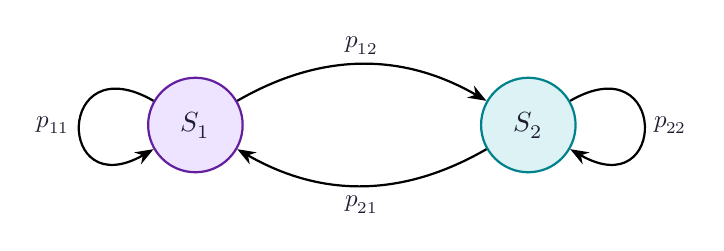
\begin{tikzpicture}[node distance=2.5cm,>=Stealth,auto,thick]
  % Nodes representing states
  \node[circle, draw=mypurple, fill=hdrpurple, minimum size=1.2cm, font=\bfseries\color{mydark}] (S1) {$S_1$};
  \node[circle, draw=myteal, fill=hdrteal, minimum size=1.2cm, right=3.0cm of S1, font=\bfseries\color{mydark}] (S2) {$S_2$};

  % Transition arrows
  \path[->] 
    (S1) edge [bend left=30] node[above, font=\small\color{mydark}] {$p_{12}$} (S2)
    (S2) edge [bend left=30] node[below, font=\small\color{mydark}] {$p_{21}$} (S1)
    (S1) edge [loop left, out=150, in=210, looseness=6] node[left, font=\small\color{mydark}] {$p_{11}$} (S1)
    (S2) edge [loop right, out=30, in=330, looseness=6] node[right, font=\small\color{mydark}] {$p_{22}$} (S2);
\end{tikzpicture}
\end{tcolorbox}

\subsection{Transition Probability Matrix (TPM)}
The transition probabilities of a Markov chain with $K$ states are organized into a square matrix $P$:
\begin{equation}
  P = \begin{bmatrix}
    p_{11} & p_{12} & \dots & p_{1K} \\
    p_{21} & p_{22} & \dots & p_{2K} \\
    \vdots & \vdots & \ddots & \vdots \\
    p_{K1} & p_{K2} & \dots & p_{KK}
  \end{bmatrix}
\end{equation}
Since the source must transition to one of the possible states, the sum of probabilities in each row is exactly 1:
\begin{equation}
  \sum_{j=1}^K p_{ij} = 1 \quad \text{for all } i = 1, 2, \dots, K
\end{equation}

\subsection{Stationary State Probabilities}
Let $\mathbf{W} = [w_1, w_2, \dots, w_K]$ represent the stationary (steady-state) probability vector, where $w_i$ is the probability that the source is in state $i$ in the long run.
\begin{tcolorbox}[formulabox, title={\textbf{Stationary State Probability Equations}}]
The stationary probability vector satisfies:
\begin{equation}
  \mathbf{W} P = \mathbf{W} \quad \text{and} \quad \sum_{i=1}^K w_i = 1
\end{equation}
Which yields a system of linear equations:
\begin{align}
  w_1 p_{11} + w_2 p_{21} + \dots + w_K p_{K1} &= w_1 \\
  w_1 p_{12} + w_2 p_{22} + \dots + w_K p_{K2} &= w_2 \\
  &\;\; \vdots \\
  w_1 + w_2 + \dots + w_K &= 1
\end{align}
\end{tcolorbox}

\subsection{Entropy of Markov Sources (Entropy Rate)}
Because the output probability depends on the current state, we first calculate the entropy of each state individually, and then compute the weighted average over all states.
\begin{tcolorbox}[formulabox, title={\textbf{Markov Source Entropy Rate Formulas}}]
\begin{enumerate}[label=\textbf{\arabic*.}, leftmargin=1.5em, itemsep=4pt, topsep=2pt]
  \item \textbf{Entropy of State $i$ ($H_i$):} The uncertainty of the next symbol given the source is currently in state $i$.
    \begin{equation}
      H_i = -\sum_{j=1}^K p_{ij} \log_2 p_{ij} \quad (\text{bits/symbol})
    \end{equation}
  \item \textbf{Average Entropy of Markov Source ($H(X)$):} The long-run average uncertainty per symbol.
    \begin{equation}
      H(X) = \sum_{i=1}^K w_i H_i = -\sum_{i=1}^K w_i \sum_{j=1}^K p_{ij} \log_2 p_{ij} \quad (\text{bits/symbol})
    \end{equation}
\end{enumerate}
\end{tcolorbox}

\begin{tcolorbox}[examplebox, title={Worked Example: Entropy Rate of a Markov Source}]
\textbf{Problem:} A 2-state Markov source has the following transition probability matrix:
\begin{equation*}
  P = \begin{bmatrix}
    0.8 & 0.2 \\
    0.3 & 0.7
  \end{bmatrix}
\end{equation*}
\begin{enumerate}[label=\alph*., leftmargin=*, itemsep=1pt, topsep=1pt]
  \item Find the stationary state probabilities $w_1$ and $w_2$.
  \item Calculate the state entropies $H_1$ and $H_2$.
  \item Find the average entropy rate $H(X)$ of this source.
\end{enumerate}
\textbf{Solution:}

\textbf{(a) Find stationary probabilities $w_1$ and $w_2$:}
Using $\mathbf{W}P = \mathbf{W}$:
\begin{equation*}
  [w_1, w_2] \begin{bmatrix} 0.8 & 0.2 \\ 0.3 & 0.7 \end{bmatrix} = [w_1, w_2]
\end{equation*}
This yields the equations:
\begin{align*}
  0.8w_1 + 0.3w_2 &= w_1 \implies 0.3w_2 = 0.2w_1 \implies w_2 = \frac{2}{3}w_1 \\
  0.2w_1 + 0.7w_2 &= w_2 \implies 0.2w_1 = 0.3w_2 \quad (\text{redundant})
\end{align*}
Using the probability normalization constraint $w_1 + w_2 = 1$:
\begin{equation*}
  w_1 + \frac{2}{3}w_1 = 1 \implies \frac{5}{3}w_1 = 1 \implies w_1 = 0.6 \quad \text{and} \quad w_2 = 0.4
\end{equation*}

\textbf{(b) Calculate state entropies $H_1$ and $H_2$:}
\begin{align*}
  H_1 &= -[0.8\log_2 0.8 + 0.2\log_2 0.2] = -[0.8(-0.3219) + 0.2(-2.3219)] = 0.7219 \text{ bits/symbol} \\
  H_2 &= -[0.3\log_2 0.3 + 0.7\log_2 0.7] = -[0.3(-1.7370) + 0.7(-0.5146)] = 0.8813 \text{ bits/symbol}
\end{align*}

\textbf{(c) Find the average entropy rate $H(X)$:}
\begin{align*}
  H(X) &= w_1 H_1 + w_2 H_2 \\
  &= (0.6 \times 0.7219) + (0.4 \times 0.8813) \\
  &= 0.4331 + 0.3525 = 0.7856 \text{ bits/symbol}
\end{align*}
\textbf{Answer:} $w_1=0.6, w_2=0.4$; $H_1=0.7219, H_2=0.8813$ bits/sym; average entropy is \textbf{0.7856 bits/symbol}.
\end{tcolorbox}

% ===============================================================================
\section{Shannon's Second Theorem (Noisy Channel Coding Theorem)}
% ===============================================================================

When transmitting data over physical media, noise corrupts signals, causing bit errors. Shannon proved that error-free communication is possible even over noisy channels, provided the transmission rate does not exceed a threshold called \textbf{Channel Capacity}.

\subsection{Channel Capacity Concept}
\begin{tcolorbox}[defbox]
\textbf{Channel Capacity ($C$):} The maximum rate at which information can be transmitted reliably through a communication channel. It is mathematically defined as the maximum of the mutual information $I(X; Y)$ over all possible input probability distributions $P(x)$:
\begin{equation}
  C = \max_{P(x)} I(X; Y) \quad (\text{bits/channel-use})
\end{equation}
\end{tcolorbox}

\subsection{Noisy Channel Coding Theorem}
\begin{tcolorbox}[exambox, title={\textbf{Shannon's Second Theorem (Noisy Channel Coding Theorem)}}]
Let a discrete memoryless channel have capacity $C$.
\begin{enumerate}[label=\textbf{\arabic*.}, leftmargin=1.5em, itemsep=3pt, topsep=1pt]
  \item \textbf{Theorem:} If the source transmission rate $R$ (bits/second) is less than or equal to $C$ ($R \le C$), there exists a coding scheme (with block length $N$ sufficiently large) such that the probability of error at the receiver, $P_e$, can be made arbitrarily small:
    \begin{equation}
      \lim_{N \to \infty} P_e = 0
    \end{equation}
  \item \textbf{Converse:} If $R > C$, it is impossible to design a coding scheme that achieves error-free transmission. The probability of bit error $P_e$ is bounded away from zero, and reliable communication cannot occur.
\end{enumerate}
\end{tcolorbox}

This theorem is historically significant because it proved that channel noise limits the \textbf{rate of transmission}, not its \textbf{accuracy}. We do not need noiseless channels for error-free data transfer; we only need appropriate error-correcting codes.

% ===============================================================================
\section{Calculation of Channel Capacity for Discrete Channels}
% ===============================================================================

A discrete channel is represented by input alphabet $X$, output alphabet $Y$, and a channel transition matrix containing conditional probabilities $P(y_j|x_i)$.

\subsection{Binary Symmetric Channel (BSC)}
The BSC is the most common model for binary transmission. The input and output alphabets are binary $\{0, 1\}$. The probability of a bit being transmitted correctly is $1-p$, and the probability of a bit being flipped (error) is $p$.

\begin{tcolorbox}[tikzbox, title={Binary Symmetric Channel (BSC) Transition Model}]
\centering
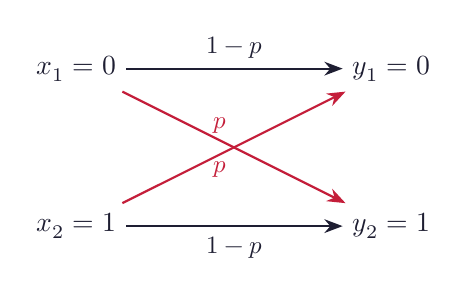
\begin{tikzpicture}[node distance=3.0cm, thick]
  % Inputs
  \node (X0) at (0, 2) [font=\bfseries\color{mydark}] {$x_1 = 0$};
  \node (X1) at (0, 0) [font=\bfseries\color{mydark}] {$x_2 = 1$};

  % Outputs
  \node (Y0) at (4, 2) [font=\bfseries\color{mydark}] {$y_1 = 0$};
  \node (Y1) at (4, 0) [font=\bfseries\color{mydark}] {$y_2 = 1$};

  % Transition arrows
  \draw[arrow] (X0) -- (Y0) node[midway, above, font=\small\color{myteal}] {$1-p$};
  \draw[arrow] (X1) -- (Y1) node[midway, below, font=\small\color{myteal}] {$1-p$};
  \draw[redarrow] (X0) -- (Y1) node[pos=0.3, right=5pt, font=\small\color{myred}] {$p$};
  \draw[redarrow] (X1) -- (Y0) node[pos=0.3, right=5pt, font=\small\color{myred}] {$p$};
\end{tikzpicture}
\tcbset{colbacktitle=myteal, coltitle=white}
\end{tcolorbox}

\subsubsection{Derivation of BSC Channel Capacity}
We calculate capacity using $I(X; Y) = H(Y) - H(Y|X)$.
First, evaluate the conditional entropy $H(Y|X)$:
\begin{align*}
  H(Y|X) &= -\sum_{i=1}^2 P(x_i) \sum_{j=1}^2 P(y_j|x_i) \log_2 P(y_j|x_i) \\
  &= -P(x_1) \left[ P(y_1|x_1)\log_2 P(y_1|x_1) + P(y_2|x_1)\log_2 P(y_2|x_1) \right] \\
  &\quad - P(x_2) \left[ P(y_1|x_2)\log_2 P(y_1|x_2) + P(y_2|x_2)\log_2 P(y_2|x_2) \right] \\
  &= -P(x_1) \left[ (1-p)\log_2(1-p) + p\log_2 p \right] - P(x_2) \left[ p\log_2 p + (1-p)\log_2(1-p) \right]
\end{align*}
Since $P(x_1) + P(x_2) = 1$:
\begin{equation*}
  H(Y|X) = -p\log_2 p - (1-p)\log_2(1-p) = H(p) \quad (\text{independent of input distribution } P(x))
\end{equation*}
Substitute this into the capacity equation:
\begin{equation*}
  C = \max_{P(x)} \left[ H(Y) - H(Y|X) \right] = \max_{P(x)} H(Y) - H(p)
\end{equation*}
Since $Y$ is a binary variable, its entropy $H(Y)$ is maximized when $Y$ has equiprobable outputs, i.e., $P(y_1) = P(y_2) = 0.5$, which yields $H(Y)_{\text{max}} = 1$. This maximum is achieved when the input symbols are equiprobable ($P(x_1) = P(x_2) = 0.5$).
\begin{tcolorbox}[formulabox, title={\textbf{BSC Channel Capacity}}]
\begin{equation}
  C_{\text{BSC}} = 1 - H(p) = 1 + p\log_2 p + (1-p)\log_2(1-p) \quad (\text{bits/channel-use})
\end{equation}
\end{tcolorbox}

\subsection{Binary Erasure Channel (BEC)}
In a BEC, the transmitter sends binary digits $\{0, 1\}$. Due to noise, the receiver may fail to decode the bit. Rather than receiving an incorrect bit, the receiver recognizes a lost bit and labels it as an erasure symbol '$e$'. The probability of erasure is $\alpha$.

\begin{tcolorbox}[tikzbox, title={Binary Erasure Channel (BEC) Transition Model}]
\centering
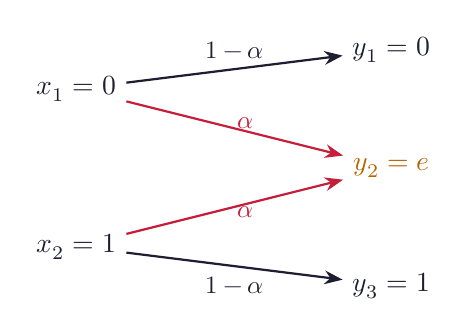
\begin{tikzpicture}[node distance=3.0cm, thick]
  % Inputs
  \node (X0) at (0, 2.5) [font=\bfseries\color{mydark}] {$x_1 = 0$};
  \node (X1) at (0, 0.5) [font=\bfseries\color{mydark}] {$x_2 = 1$};

  % Outputs
  \node (Y0) at (4, 3) [font=\bfseries\color{mydark}] {$y_1 = 0$};
  \node (Ye) at (4, 1.5) [font=\bfseries\color{myamber}] {$y_2 = e$};
  \node (Y1) at (4, 0) [font=\bfseries\color{mydark}] {$y_3 = 1$};

  % Transition arrows
  \draw[arrow] (X0) -- (Y0) node[midway, above, font=\small\color{myteal}] {$1-\alpha$};
  \draw[arrow] (X1) -- (Y1) node[midway, below, font=\small\color{myteal}] {$1-\alpha$};
  \draw[redarrow] (X0) -- (Ye) node[pos=0.4, right=5pt, font=\small\color{myred}] {$\alpha$};
  \draw[redarrow] (X1) -- (Ye) node[pos=0.4, right=5pt, font=\small\color{myred}] {$\alpha$};
\end{tikzpicture}
\tcbset{colbacktitle=myteal, coltitle=white}
\end{tcolorbox}

\subsubsection{Capacity of the BEC}
Let the input probability be $P(x=0) = \beta$, and $P(x=1) = 1-\beta$.
The output probabilities are:
\begin{align*}
  P(y=0) &= (1-\alpha)\beta \\
  P(y=e) &= \alpha\beta + \alpha(1-\beta) = \alpha \\
  P(y=1) &= (1-\alpha)(1-\beta)
\end{align*}
To find capacity, we compute conditional entropy $H(Y|X)$:
Since for any input $x$, the output is correct with probability $1-\alpha$ and erased with probability $\alpha$:
\begin{equation*}
  H(Y|X) = H(\alpha) = -\alpha \log_2 \alpha - (1-\alpha)\log_2(1-\alpha)
\end{equation*}
The output entropy $H(Y)$ is:
\begin{align*}
  H(Y) &= -P(y=0)\log_2 P(y=0) - P(y=e)\log_2 P(y=e) - P(y=1)\log_2 P(y=1) \\
  &= -(1-\alpha)\beta \log_2 \left[(1-\alpha)\beta\right] - \alpha\log_2 \alpha - (1-\alpha)(1-\beta)\log_2 \left[(1-\alpha)(1-\beta)\right] \\
  &= -\alpha\log_2 \alpha - (1-\alpha)\log_2(1-\alpha) + (1-\alpha)\left[ -\beta\log_2\beta - (1-\beta)\log_2(1-\beta) \right] \\
  &= H(\alpha) + (1-\alpha) H(X)
\end{align*}
Using $I(X; Y) = H(Y) - H(Y|X)$:
\begin{equation*}
  I(X; Y) = H(\alpha) + (1-\alpha)H(X) - H(\alpha) = (1-\alpha)H(X)
\end{equation*}
To maximize $I(X; Y)$, we maximize $H(X)$. Since $X$ is binary, its maximum entropy is $H(X)_{\text{max}} = 1$ bit (at $\beta = 0.5$).
\begin{tcolorbox}[formulabox, title={\textbf{BEC Channel Capacity}}]
\begin{equation}
  C_{\text{BEC}} = 1 - \alpha \quad (\text{bits/channel-use})
\end{equation}
\end{tcolorbox}
This shows that erasures reduce capacity linearly: if $20\%$ of bits are erased ($\alpha = 0.2$), the capacity is $80\%$ of a noiseless channel ($C = 0.8$ bits/use).

% ===============================================================================
\section{Application to Continuous Channels}
% ===============================================================================

Discrete channel models fail when signals are continuous voltage waveforms corrupted by additive white Gaussian noise (AWGN). We analyze these systems using continuous capacities.

\subsection{The Shannon-Hartley Theorem}
\begin{tcolorbox}[defbox]
\textbf{Shannon-Hartley Theorem:} The maximum rate of transmission over a continuous channel of bandwidth $B$ (Hz), corrupted by Additive White Gaussian Noise (AWGN) with signal power $S$ and noise power $N$, is:
\begin{equation}
  C = B \log_2 \left( 1 + \frac{S}{N} \right) \quad (\text{bits/second})
\end{equation}
\end{tcolorbox}
If noise spectral density is $N_0/2$ (double-sided) or $N_0$ (single-sided), the total noise power is $N = N_0 B$:
\begin{equation}
  C = B \log_2 \left( 1 + \frac{S}{N_0 B} \right)
\end{equation}

\subsection{Implications of Shannon-Hartley Theorem}
This relation highlights several trade-offs:
\begin{enumerate}[label=\textbf{\alph*.}, leftmargin=*, itemsep=3.5pt]
  \item \textbf{Signal-to-Noise Ratio (SNR) vs Bandwidth ($B$):} We can exchange bandwidth for SNR. A system with small bandwidth can achieve high capacity if the SNR is high, and vice-versa.
  \item \textbf{Infinite Bandwidth capacity limit:} If we keep signal power $S$ and noise density $N_0$ constant, and let the bandwidth $B$ grow to infinity, the capacity does not grow to infinity. Instead, it reaches a thermodynamic limit:
\end{enumerate}

\subsubsection{Derivation of Infinite Bandwidth Capacity}
We evaluate the limit of $C$ as $B \to \infty$:
\begin{equation*}
  \lim_{B \to \infty} C = \lim_{B \to \infty} B \log_2 \left( 1 + \frac{S}{N_0 B} \right)
\end{equation*}
Let $x = \frac{S}{N_0 B}$. As $B \to \infty$, $x \to 0$. We express $B$ as $B = \frac{S}{N_0 x}$:
\begin{align*}
  \lim_{B \to \infty} C &= \lim_{x \to 0} \frac{S}{N_0 x} \log_2 (1 + x) \\
  &= \frac{S}{N_0} \lim_{x \to 0} \log_2 (1 + x)^{1/x}
\end{align*}
By the definition of the natural base $e$, $\lim_{x \to 0} (1+x)^{1/x} = e$:
\begin{equation*}
  \lim_{B \to \infty} C = \frac{S}{N_0} \log_2 e \approx 1.4427 \frac{S}{N_0}
\end{equation*}
\begin{tcolorbox}[formulabox, title={\textbf{Infinite Bandwidth Capacity Limit}}]
\begin{equation}
  C_{\infty} = 1.44 \frac{S}{N_0} \quad (\text{bits/second})
\end{equation}
\end{tcolorbox}
This represents the absolute physical limit on transmission capacity under a power constraint, even with infinite bandwidth.

\subsection{Bandwidth-Efficiency Trade-off ($C/B$ vs. $E_b/N_0$)}
We define the \textbf{spectral efficiency} as $C/B$ (bps/Hz). Let $E_b$ be the energy per bit transmitted. Since signal power is energy per unit time:
\begin{equation*}
  S = C \times E_b
\end{equation*}
Substitute this into the Shannon-Hartley equation:
\begin{align*}
  \frac{C}{B} &= \log_2 \left( 1 + \frac{C E_b}{B N_0} \right) \\
  2^{C/B} &= 1 + \frac{C}{B} \left(\frac{E_b}{N_0}\right)
\end{align*}
Solving for $E_b/N_0$:
\begin{tcolorbox}[formulabox, title={\textbf{Bandwidth-Efficiency Relation}}]
\begin{equation}
  \frac{E_b}{N_0} = \frac{2^{C/B} - 1}{C/B}
\end{equation}
\end{tcolorbox}

\subsubsection{Derivation of the Shannon Limit}
To find the absolute minimum value of $E_b/N_0$ required for error-free communication, we take the limit as the spectral efficiency $C/B \to 0$ (highly redundant coding over very wide bandwidth):
\begin{equation*}
  \lim_{C/B \to 0} \frac{E_b}{N_0} = \lim_{y \to 0} \frac{2^y - 1}{y}
\end{equation*}
Using L'H\^opital's rule (differentiating numerator and denominator with respect to $y$):
\begin{equation*}
  \lim_{y \to 0} \frac{\ln 2 \cdot 2^y}{1} = \ln 2 \approx 0.693
\end{equation*}
Expressed in decibels (dB):
\begin{equation*}
  \left(\frac{E_b}{N_0}\right)_{\text{dB}} = 10 \log_{10} (0.693) \approx -1.59 \text{ dB}
\end{equation*}
\begin{tcolorbox}[formulabox, title={\textbf{The Shannon Limit}}]
The minimum energy-to-noise ratio required for reliable transmission is:
\begin{equation}
  \left(\frac{E_b}{N_0}\right)_{\text{min}} = -1.59 \text{ dB}
\end{equation}
\end{tcolorbox}
If a system operates below $-1.59 \text{ dB}$, error-free communication is physically impossible.

\begin{tcolorbox}[tikzbox, title={Spectral Efficiency $C/B$ vs $E_b/N_0$ (Shannon Boundary)}]
\centering
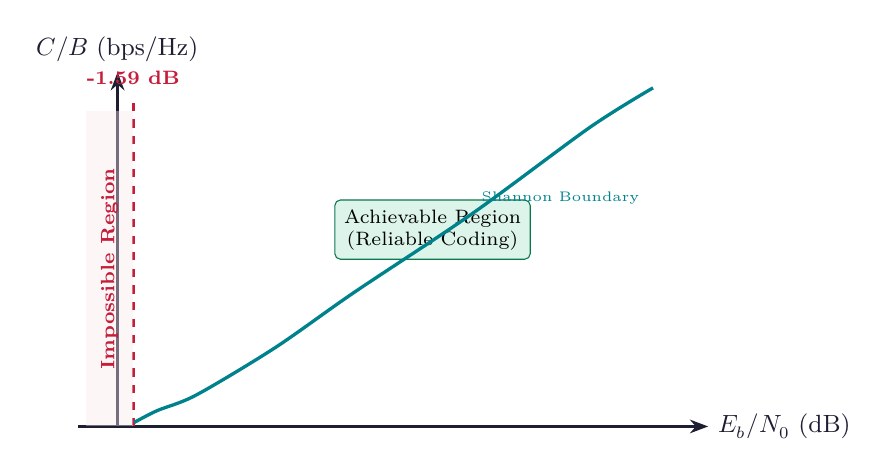
\begin{tikzpicture}
  % Draw axes
  \draw[-Stealth, thick, color=mydark] (-1.5,0) -- (6.5,0) node[right, font=\small] {$E_b/N_0$ (dB)};
  \draw[-Stealth, thick, color=mydark] (-1,0) -- (-1,4.5) node[above, font=\small] {$C/B$ (bps/Hz)};

  % Grid line for Shannon limit
  \draw[dashed, color=myred, line width=1pt] (-0.8,0) -- (-0.8,4.2) node[above, font=\scriptsize\bfseries\color{myred}] {-1.59 dB};

  % Draw shading for regions
  \fill[hdrred, opacity=0.4] (-1.4,0) rectangle (-0.8,4);
  \node[rotate=90, font=\scriptsize\bfseries\color{myred}] at (-1.1,2) {Impossible Region};
  \node[draw=mygreen, fill=hdrgreen, rounded corners=2pt, font=\scriptsize, align=center] at (3,2.5) {Achievable Region\\(Reliable Coding)};

  % Plot Shannon capacity limit curve
  % Coordinates scaled: dB = -1.6 -> x=-0.8, dB=0 -> x=0.5, dB=5 -> x=2.5, dB=10 -> x=5.0
  % C/B = 0 -> y=0, C/B = 1 -> y=1, C/B = 2 -> y=2.2, C/B = 4 -> y=3.8
  \draw[very thick, color=myteal, smooth] plot coordinates {
    (-0.79, 0.05) (-0.5, 0.2) (0.0, 0.4) (1.0, 1.0) (2.0, 1.7) (3.5, 2.7) (5.0, 3.8) (5.8, 4.3)
  };

  \node[right, font=\tiny\color{myteal}] at (3.5,2.9) {Shannon Boundary};
\end{tikzpicture}
\end{tcolorbox}

% ===============================================================================
% MANDATORY QUICK REVISION PAGE
% ===============================================================================
\newpage
\begin{center}
  {\large\bfseries\color{myred} Quick Revision --- Module II}\\[3pt]
  {\small\color{mydark} Markov Sources \& Channel Capacity $|$ PE-EC603D}
\end{center}
\noindent{\color{myred}\rule{\linewidth}{1.2pt}}
\vspace{4pt}

\begin{tcolorbox}[formulabox, title={\textbf{Key Formulas at a Glance}}]
\renewcommand{\arraystretch}{1.3}
\begin{tabularx}{\linewidth}{B{4.5cm} X}
Markov Transition Prob.  & $\sum_{j=1}^K p_{ij} = 1 \quad (\text{Row sum of TPM equals 1})$ \\[4pt]
Steady-State Vector     & $\mathbf{W}P = \mathbf{W} \quad \text{and} \quad \sum w_i = 1$ \\[4pt]
State Entropy           & $H_i = -\sum_{j=1}^K p_{ij} \log_2 p_{ij}$ \\[4pt]
Markov Source Entropy   & $H(X) = \sum w_i H_i$ \\[4pt]
Channel Capacity        & $C = \max_{P(x)} I(X;Y) \quad (\text{bits/channel-use})$ \\[4pt]
BSC Capacity            & $C_{\text{BSC}} = 1 - H(p) = 1 + p\log_2 p + (1-p)\log_2(1-p)$ \\[4pt]
BEC Capacity            & $C_{\text{BEC}} = 1 - \alpha$ \\[4pt]
Shannon-Hartley Theorem & $C = B \log_2 \left( 1 + \frac{S}{N} \right) = B \log_2 \left( 1 + \frac{S}{N_0 B} \right)$ (bps) \\[4pt]
Infinite Bandwidth Limit & $C_{\infty} = 1.44 \frac{S}{N_0}$ \\[4pt]
Shannon Limit (Min SNR) & $\left(\frac{E_b}{N_0}\right)_{\text{min}} = \ln 2 \approx 0.693 \approx -1.59 \text{ dB}$
\end{tabularx}
\end{tcolorbox}

\begin{tcolorbox}[defbox, title={\textbf{One-Line Definitions}}]
\begin{itemize}[leftmargin=*, itemsep=2.5pt, topsep=0pt]
  \item \textbf{Markov Source:} A source with memory where current output statistics depend on previous state history.
  \item \textbf{Transition Matrix (TPM):} A matrix storing conditional probabilities of moving between Markov states.
  \item \textbf{Steady-State Vector:} Stationary probabilities indicating long-run occupancy rates of Markov states.
  \item \textbf{Channel Capacity:} The maximum rate of information transmission that can be achieved over a channel.
  \item \textbf{Binary Symmetric Channel:} A binary channel model with symmetric error (crossover) probability $p$.
  \item \textbf{Binary Erasure Channel:} A channel model where bits are either received correctly or recognized as lost (erased).
  \item \textbf{AWGN Channel:} A continuous channel model corrupted by additive white Gaussian noise.
  \item \textbf{Shannon Limit:} The absolute minimum value of $E_b/N_0$ ($-1.59\text{ dB}$) required for error-free transmission.
\end{itemize}
\end{tcolorbox}

\begin{tcolorbox}[exambox, title={\textbf{Frequently Asked / Viva Questions}}]
\begin{enumerate}[topsep=0pt, label=\textbf{Q\arabic*.}, itemsep=5pt]
  \item \Q{State the main condition that defines a first-order Markov source.}
    The output probability at any time instant depends only on the output symbol of the immediately preceding time instant.
  \item \Q{Why does the sum of transition probabilities in each row of a TPM equal 1?}
    A row represents all transition possibilities leaving a specific state. The source must transition to one of the possible states, so the sum of these probabilities is certain (1).
  \item \Q{Explain the physical meaning of Shannon's Second Theorem.}
    If transmission rate $R \le C$, error-free communication is possible using coding. If $R > C$, it is physically impossible to achieve error-free communication.
  \item \Q{What happens to the capacity of a BSC when the crossover probability $p = 0.5$?}
    Capacity $C = 1 - H(0.5) = 1 - 1 = 0$. The channel output is completely random and independent of input, meaning no information can be transmitted.
  \item \Q{What is an "erasure" symbol in the context of a BEC?}
    It is a symbol received as a lost bit (labeled '$e$'), meaning the receiver knows a bit was sent but cannot determine if it was '0' or '1'.
  \item \Q{What are the components of noise in the Shannon-Hartley theorem?}
    Additive (noise is added to signal), White (flat power spectral density across all frequencies), and Gaussian (probability density function of noise voltage is Gaussian).
  \item \Q{Why can't we achieve infinite channel capacity by making the bandwidth infinite?}
    As bandwidth increases, the noise power $N = N_0 B$ also increases. The capacity reaches a thermodynamic limit of $1.44 S/N_0$ bps.
  \item \Q{Explain the bandwidth-SNR trade-off using a practical example.}
    In telephone channels with small bandwidth, high SNR is used to achieve high rates. In satellite links with low power (low SNR), wide bandwidths are used.
  \item \Q{State the value of the Shannon Limit and its practical significance.}
    $-1.59 \text{ dB}$. It is the absolute minimum signal-to-noise ratio per bit required to transmit information over an AWGN channel without errors.
  \item \Q{Under what conditions does the capacity of a channel equal its bandwidth?}
    When the signal-to-noise ratio $S/N = 1$ (or $0 \text{ dB}$), because $C = B \log_2(1+1) = B \log_2(2) = B$ bps.
  \item \Q{Distinguish between a lossless channel and a noiseless channel.}
    In a lossless channel, $H(Y|X) = 0$ (no noise, inputs map uniquely to outputs). In a noiseless channel, $H(X|Y) = 0$ (outputs map uniquely to inputs, no ambiguity).
  \item \Q{How do you calculate the entropy of a Markov source?}
    First, find steady-state probabilities $\mathbf{W}$. Then, calculate state entropies $H_i$. The average source entropy is the weighted sum $H(X) = \sum w_i H_i$.
\end{enumerate}
\tcbset{colbacktitle=mypurple, coltitle=white}
\end{tcolorbox}

\begin{tcolorbox}[tikzbox, title={Comparison of BSC and BEC Models}]
\renewcommand{\arraystretch}{1.45}
\par\noindent
\begin{tabularx}{\linewidth}{|B{3.2cm}|Y|Y|}
\hline
\textbf{Parameter} & \textbf{\color{myteal}Binary Symmetric Channel (BSC)} & \textbf{\color{mygreen}Binary Erasure Channel (BEC)} \\
\hline
\textbf{Input Alphabet} & Binary: $\{0, 1\}$ & Binary: $\{0, 1\}$ \\
\hline
\textbf{Output Alphabet} & Binary: $\{0, 1\}$ & Ternary: $\{0, e, 1\}$ (where $e$ is erasure) \\
\hline
\textbf{Error Type} & Bit flip (crossover), $0 \leftrightarrow 1$. & Bit loss, input becomes unreadable symbol $e$. \\
\hline
\textbf{Error Knowledge} & Receiver does not know which bits are flipped. & Receiver knows exactly which bits are erased. \\
\hline
\textbf{Capacity Formula} & $C = 1 - H(p)$ bits/use & $C = 1 - \alpha$ bits/use \\
\hline
\end{tabularx}
\end{tcolorbox}

\end{document}
